\chapter{Register File}

\section{Register File}

Next, we will create the register file.  You will create a new module called regfile (in regfile.v), and this module will be part of your iDecode module.  The regfile module should retrieve data from the registers as well as write to the registers when the regWrite flag is set and the clock edge rises.  The regfile should use a verilog reg array.  You do not need to use the register module that you used for your program counter.  Since we don't currently have the ability to do loads and stores (since we don't have data memory yet), the values for the registers should be stored in a datafile, fibR.data and read in during the initial block.  In order to get results that match my provided results (and match the provided unit test), you should set X21=16, X9=33, X10=12 in fibR.data.

A unit test is provided, iDecode\_test.v.  It simply sends two commands (the add and subtract commands from last lab) and sets a few flags.  Using that unit test, you should be able to produce the results shown in the lab manual.  Note that in addition to the register file, you will also need to create a mux to determine the source of the second read register.  Note that because we are sending the instructions from the test instead of from the iFetch routine, you will need to update your code from last lab to use procedural statements triggered on the clock edge.  Otherwise, the instructions will not come in on the clock edge as expected.  Timing is very important in this lab.

\begin{figure}
	\caption{Expected Results}\label{fig:register_file_cutout}
	\begin{center}
		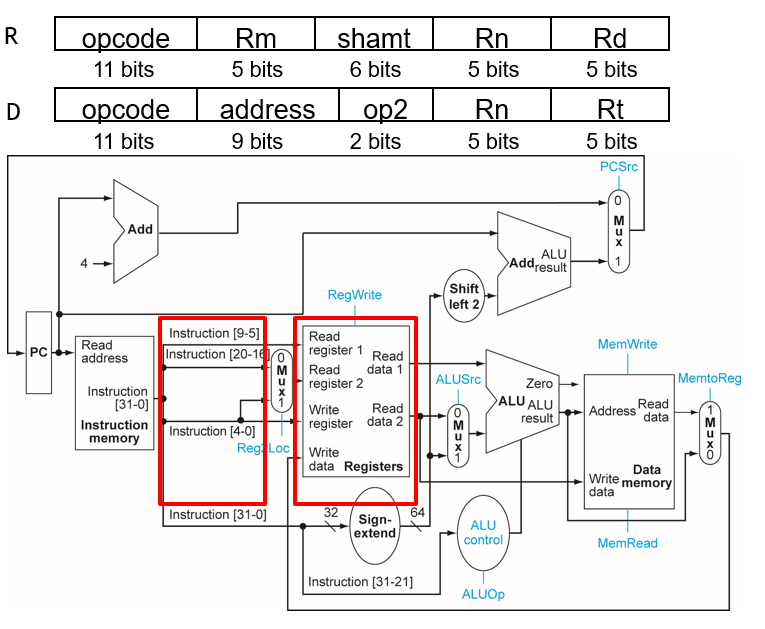
\includegraphics[width=4.75in]{../images/register_file_cutout.png}
	\end{center}
\end{figure} 

\Verilog{Verilog starter code for the iDecode module.}{code:iDecode_reg_test_version}{../code/2_decode/iDecode_reg_test_version.v}

\begin{figure}
	\caption{Expected Results}\label{fig:register_file_test_output}
	\begin{center}
		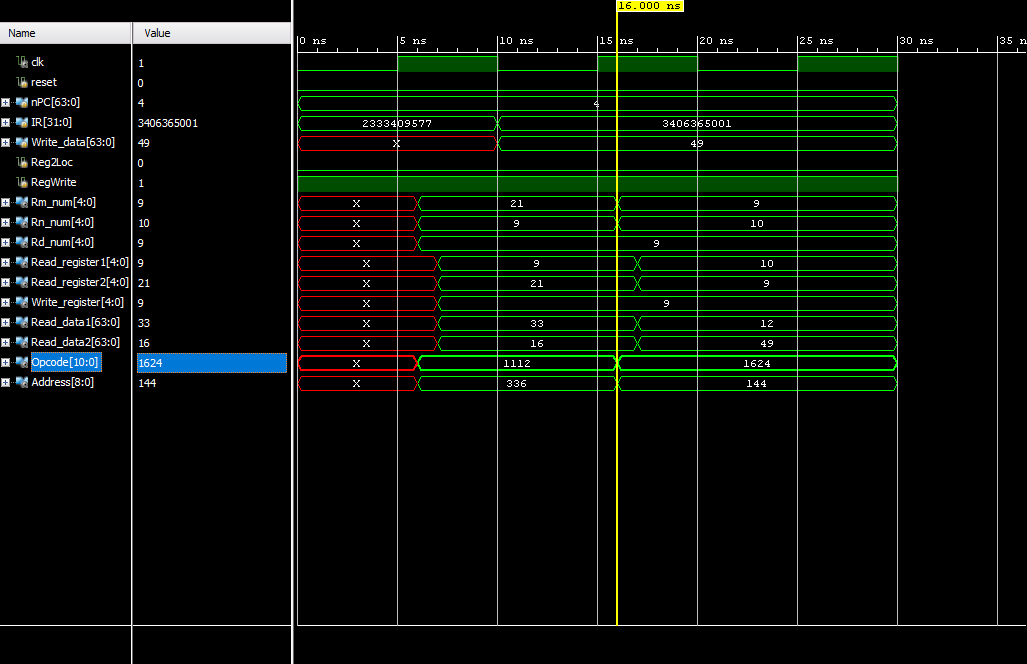
\includegraphics[width=6.75in]{../images/register_file_test_output.png}
	\end{center}
\end{figure}

\clearpage
\section{Your Assignment}

You are to:
\begin{enumerate}
\item Create a regfile module and add it to the iDecode module.
\item Re-use your mux from previous labs and add it to the iDecode module.
\item Import the provided iDecode\_test.v file.
\item Verify that your results match the expected results.
\item There will not be a submittal on Canvas today.  However, please show me your results either today or at the beginning of lab time during the next class period.  We will be adding more functionality next time.
\end{enumerate} 